\section{API}
Die Webapplikation kommuniziert mit dem Server über ein \gls{rest} \gls{api}.

\subsection{Konzepte}
Folgende Konzepte werden von mehreren Endpunkten verwendet und werden daher separat aufgelistet.

\subsubsection{Paging} \label{sec:pd:api-paging} 
Paging ermöglicht das limitieren der Anzahl Resultate, welche eine Abfrage liefert. Die Einträge pro Seite werden mit dem Parameter \texttt{count} gesteuert, die Seite mit \texttt{page}.

\subsubsection{Suche} \label{sec:pd:api-search} 
Für die Suche werden folgende Parameter verwendet:
\mytable{lX}{
  \textbf{Parameter} & \textbf{Beschreibung}  \\
  \midrule
  \textbf{filter[name]} & Filtert anhand des Namens \\
  \textbf{filter[description]} & Filtert anhand der Beschreibung \\
  \textbf{filter[search]} & Filtert sowohl mit Namen als auch mit der Beschreibung \\
  \textbf{filter[mineOnly]} & Liefert nur Dokumente, die dem eingeloggten Benutzer zugeordnet sind \\
}{Such-Parameter}{pd:api-search}

\subsubsection{Sortierung} \label{sec:pd:api-sort}
Sortiert die Resultate der Anfrage. Dazu kann der Parameter \texttt{sorting[key]=asc|desc} verwendet werden, mit folgenden Werten als \texttt{key}: \texttt{name}, \texttt{description}, \texttt{private}, \texttt{owner} und \texttt{created\_at}.

\paragraph{Preview} \label{sec:pd:api-preview}
Liefert eine Vorschau der Daten. Enthalten ist der Unique Name, welcher in Abfragen verwendet werden kann, eine Liste der Felder und deren Typen sowie ein paar Daten-Zeilen. Die Anzahl der gelieferten Daten-Zeilen kann per Paging gesteuert werden (siehe \cref{sec:pd:api-paging}).

\begin{srclst}{json}{Preview für ein Dokument}
[  
   {  
      "type":"preview",
      "unique_name":"ODH4_Bahnhoefe",
      "parent":"4",
      "types":{  
         "TYPE":"BIGINT",
         "fid":"TEXT",
         "CNTRYNAME":"TEXT",
         "DUP_NAME":"TEXT",
         "PROV1NAME":"TEXT",
         "LEVEL":"BIGINT",
         "geometry":"GEOMETRY",
         "NATION":"BIGINT",
         "CONURB":"TEXT",
         "name":"TEXT"
      },
      "url":"http://beta.opendatahub.ch/api/v1/document/4/preview/",
      "columns":[ "TYPE", "fid", "geometry", "DUP_NAME", "PROV1NAME", "LEVEL", "CNTRYNAME", "NATION", "CONURB", "name" ],
      "data":[  
         {  
            "TYPE":"3",
            "fid":"F0",
            "CNTRYNAME":"Switzerland",
            "DUP_NAME":"N",
            "PROV1NAME":"Tessin",
            "LEVEL":"10",
            "geometry":"POINT (45.90247783251107 76645.7742365048)",
            "NATION":"41",
            "CONURB":"NULL",
            "name":"Chiasso Rail"
         },
         ...
      ],
      "count":1781,
      "name":"Bahnhoefe"
   }
]
\end{srclst}

\subsubsection{Download} \label{sec:pd:api-download}
Fordert einen Download der Daten an. Das gewünschte Format wird mit dem Parameter \texttt{fmt} angegeben. Gültige Werte sind die von \cref{sec:pd:api-format} gelieferten Namen. Ohne Format-Angabe werden die Original-Daten geliefert.

Hinweis: Dokumente können nicht als ganzes heruntergeladen werden \textendash stattdessen müssen die File Groups für diesen Zweck verwendet werden.

\subsection{Root - GET /api/v1/}
Als Prefix für die \gls{api} URLs wird \url{/api/v1/} verwendet, was eine spätere versionierte Erweiterung erlaubt.
\begin{figure}[H]
\centering
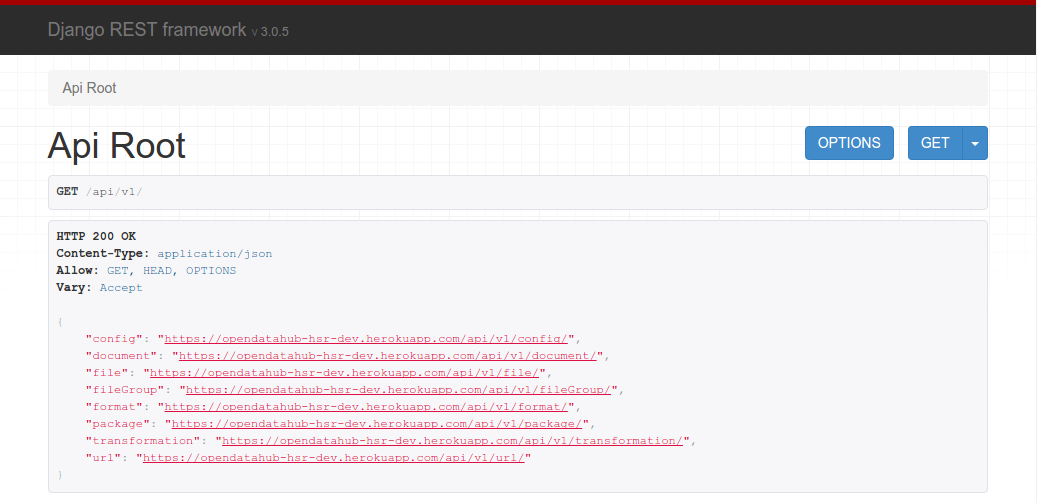
\includegraphics[width=\linewidth]{fig/api-root}
\caption{API: Übersicht}
\label{fig:pd:api-root}
\end{figure}

Da für die Implementation des \gls{api} die Django-Erweiterung \texttt{rest\_framework}\footnote{\url{http://www.django-rest-framework.org/}} verwendet wurde, kann die API gut auch manuell ausprobiert werden. Dabei ist zu beachten, dass die Schrägstriche am Ende der URLs nicht optional sind.

\subsection{Konfiguration - GET /api/v1/config/}
Gibt die für den HTML5 Client notwendigen Konfigurationsinformationen zurück.

\begin{srclst}{json}{Beispielantwort für GET /api/v1/config/}
{
  "GITHUB_PUBLIC": "8ef558ed3fb0f5385da5", 
  "FACEBOOK_PUBLIC": "401520096685508", 
  "PACKAGE_PREFIX": "ODH", 
  "TRANSFORMATION_PREFIX": "TRF"
}
\end{srclst}

\subsection{Liste der unterstützten Formate - GET /api/v1/format/} \label{sec:pd:api-format}
Liefert die Liste der unterstützten Formate. Neue Formate erscheinen automatisch, sobald sie registriert sind, vorausgesetzt dass ein Formatter für das Format existiert.

\begin{srclst}{json}{Beispielantwort für GET /api/v1/format/}
[
    {
        "name": "JSON", 
        "label": "JSON", 
        "description": "JavaScript Objekt-Notation. Nützlich zur Wiederverwendung in Webapplikationen.", 
        "example": "", 
        "extension": "json"
    }, 
    {
        "name": "GML", 
        "label": "GML", 
        "description": "Geometry Markup Language (GML) ist ein Dateiformat zum Austausch von Geodaten.", 
        "example": "", 
        "extension": "gml"
    }, 
    ...
]
\end{srclst}

\subsection{Packages}
``Package'' wird als Überbegriff für Dokumente, welche von Nutzern bereitgestellt wurden oder für Transformationen verwendet. Packages haben Attribute wie ``Name'' oder ``Beschreibung'', können eine Vorschau erzeugen und der Benutzer kann einen Download anfordern.

\subsubsection{Package-Liste - GET /api/v1/package/}\label{sec:pd:api-package-list}
Liefert eine Liste der Packages.

\begin{srclst}{json}{Beispielantwort für GET /api/v1/package/}
{
    "count": 37, 
    "next": "http://beta.opendatahub.ch/api/v1/package/?page=2", 
    "previous": null, 
    "results": [
        {
            "id": 1, 
            "url": "http://beta.opendatahub.ch/api/v1/package/1/", 
            "name": "Test mockaroo.com.csv", 
            "description": "Testdaten (Originalformat: CSV)", 
            "private": false, 
            "owner": {
                "id": 1, 
                "username": "testuser", 
                "first_name": "", 
                "last_name": ""
            }, 
            "created_at": "2015-06-01T12:35:31.480135Z", 
            "type": "document", 
            "preview": "http://beta.opendatahub.ch/api/v1/document/1/preview/", 
            "template": false
        }, 
        {
            "id": 2001, 
            "url": "http://beta.opendatahub.ch/api/v1/package/2001/", 
            "name": "TROBDB: Baustellen Februar 2015", 
            "description": "TROBDB: Baustellen Februar 2015", 
            "private": false, 
            "owner": {
                "id": 1, 
                "username": "testuser", 
                "first_name": "", 
                "last_name": ""
            }, 
            "created_at": "2015-06-01T12:35:45.794037Z", 
            "type": "transformation", 
            "preview": "http://beta.opendatahub.ch/api/v1/transformation/2001/preview/", 
            "template": false
        },
        ...
    ]
}
\end{srclst}

Dieser Endpunkt unterstützt Paging (\cref{sec:pd:api-paging}), Suche (\cref{sec:pd:api-search}) und Sortierung (\cref{sec:pd:api-sort}).

\subsubsection{Package-Details - GET /api/v1/package/<id>/}\label{sec:pd:api-package-details}
Liefert die Details zu einem Package. Dies sind grundsätzlich die selben Informationen wie in der Package-Liste, jedoch um einige weitere Details ergänzt.

Die Antwort sieht unterschiedlich aus, je nach dem ob das Package ein Dokument (\cref{pd:api-package-document}) oder eine Transformation (\cref{pd:api-package-transformation}) ist.

\begin{srclst}[label=pd:api-package-document]{json}{Beispielantwort für ein Dokument}
{
    "id": 4, 
    "url": "http://beta.opendatahub.ch/api/v1/document/4/", 
    "name": "Test Bahnhoefe.gml, Bahnhoefe.gfs, Bahnhoefe.xsd", 
    "description": "Testdaten (Originalformat: GML)", 
    "file_groups": "http://beta.opendatahub.ch/api/v1/document/4/filegroup/", 
    "private": false, 
    "owner": {
        "id": 1, 
        "username": "testuser", 
        "first_name": "", 
        "last_name": ""
    }, 
    "created_at": "2015-06-01T12:35:32.241407Z", 
    "preview": "http://beta.opendatahub.ch/api/v1/document/4/preview/", 
    "type": "document"
}
\end{srclst}

\begin{srclst}[label=pd:api-package-transformation]{json}{Beispielantwort für eine Transformation}
{
    "id": 2001, 
    "url": "http://beta.opendatahub.ch/api/v1/transformation/2001/", 
    "name": "TROBDB: Baustellen Februar 2015", 
    "description": "TROBDB: Baustellen Februar 2015", 
    "transformation": "SELECT t.\"Federführende_Stelle\" as userid,
           substring(t.Bauarbeiten, 1, 100) as title,
           t.Bauarbeiten as description,
           to_char(to_date(concat(extract(t.Dauer, '^((?:\\\\d\\\\d?\\\\.){2})'), nvl(extract(t.Dauer, '(\\\\d{4}) -'), extract(t.Dauer, '(\\\\d{4})$'))), '%d.%m.%Y'), '%Y-%m-%d') as trob_start, -- add year from end date if not present
           to_char(to_date(extract(t.Dauer, '- ([\\\\d\\\\.]+)'), '%d.%m.%Y'), '%Y-%m-%d') as trob_end,
           null as trob_interval,
           'both' as direction,
           null as diversion_advice,
           'CH' as country,
           t.Bauarbeiten as reason,
           t.Strecke as object_name,
           'street' as object_type,
           'closed' as trob_type,
           ST_SetSRID(ST_GeomFromText(CONCAT('POINT(', CAST(t.\"Zentroid X [m]\", 'text'), ' ',CAST(t.\"Zentroid Y [m]\", 'text'), ')')), 21781) as geometry
           from \"ODH8_Baustellen Februar 2015\" as t", 
    "private": false, 
    "owner": {
        "id": 1, 
        "username": "testuser", 
        "first_name": "", 
        "last_name": ""
    }, 
    "data": "http://beta.opendatahub.ch/api/v1/transformation/2001/data/", 
    "is_template": false, 
    "preview": "http://beta.opendatahub.ch/api/v1/transformation/2001/preview/", 
    "referenced_file_groups": "http://beta.opendatahub.ch/api/v1/transformation/2001/filegroups/", 
    "referenced_transformations": "http://beta.opendatahub.ch/api/v1/transformation/2001/transformations/", 
    "related_transformations": [
        {
            "id": 2007, 
            "name": "TROBDB: Alle Daten"
        }
    ], 
    "type": "transformation"
}
\end{srclst}

\paragraph{File Groups} Die \texttt{file\_group}-Url liefert die Liste der File Groups, die zu diesem Dokument gehören. Siehe auch \cref{sec:pd:api-filegroups}.

\paragraph{Preview} Die Preview-Url liefert eine Vorschau der Daten im Package. Siehe auch \cref{sec:pd:api-preview}.

\paragraph{Referenced File Groups/Transformations} Dies sind Urls für File Groups bzw. Transformations, welche in dieser Transformation verwendet wurden.

\paragraph{Template} Templates sind abstrakte Transformationen, welche als Vorlage für konkrete Transformationen dienen. Für Templates kann keine Vorschau erstellt werden.

\paragraph{Data} Url für den Download der Daten. Siehe \cref{sec:pd:api-download} für Details.

\subsection{Dokumente}
\subsubsection{Dokument-Liste - GET /api/v1/document/}
Die Dokument-Liste ist identisch zur Package-Liste, mit der Ausnahme, dass nur Dokumente aufgeführt werden. Siehe \cref{sec:pd:api-package-list} für Details.

\subsubsection{Dokument-Details - GET /api/v1/document/<id>/} \label{sec:pd:api-document-details}
Identisch zu Package-Details, mit der Ausnahme, das nur Dokumente unterstützt werden. Siehe \cref{sec:pd:api-package-details} für Details.

\subsubsection{Dokument-Erstellung - POST /api/v1/document/}
Erstellt ein neues Dokument. 

\cref{tab:pd:api-document-offer} führt die erwarteten Parameter auf.
\mytable{lX}{
  \textbf{Parameter} & \textbf{Beschreibung} \\
  \midrule
  \textbf{name} & Dokument-Name (max. 200 Zeichen). \\
  \textbf{description} & Beschreibung des Dokuments (keine Limitation). \\
  \textbf{private} (default: false) & Steuert ob das Dokument für andere Benutzer sichtbar ist.\\
  \textbf{format} (default: null) & Format der hochgeladenen Daten. Wenn nicht angegeben wird versucht, das Format automatisch zu erkennen. \\
}{Parameter für Dokument-Erstellung}{tab:pd:api-document-offer}
\xxx[fix cref]
Zusätzlich wird eine der folgenden Optionen benötigt:
\begin{description}
\item[file] Direkter Datei-Upload. In diesem Fall wird die Anfrage als Multipart Form Request erwartet. Es kann mehr als eine Datei auf einmal hochgeladen werden. Diese werden dann dem selben Dokument zugeordnet, nach Datei-Namen (ohne Erweiterung) in File Groups gruppiert.
\item[url] Erstellt ein Dokument mit einer Url als Datenquelle. Dies kann entweder ein \gls{wfs}-Endpoint oder eine http-Url sein. Zusätzlich kann der Parameter \texttt{refresh} angegeben werden, welcher steuert wie oft die Daten abgerufen werden sollen (in Sekunden). Erlaubt sind Werte von 60 (1 Minute) bis 604800 (1 Woche).
\end{description}

\begin{srclst}{json}{Beispielanfrage für POST /api/v1/document/}
{
  "name":"aasdfas",
  "description":"asdfasdf",
  "url":"http://maps.zh.ch/wfs/TbaBaustellenZHWFS",
  "refresh":3600
}
\end{srclst}

\subsubsection{Dokument-Update - PATCH /api/v1/document/<id>/}
Aktualisiert ein Dokument. Es gelten folgende Einschränkungen:
\begin{itemize}
\item Nur die Meta-Daten (Name, Beschreibung, Privat) können aktualisiert werden.
\item Nur der Eigentümer eines Dokuments kann aktualisieren.
\end{itemize}
\subsection{Transformationen}
\subsubsection{Transformations-Liste - GET /api/v1/transformation/}
Die Transformations-Liste ist identisch zur Package-Liste, mit der Ausnahme, dass nur Transformationen aufgeführt werden. Siehe \cref{sec:pd:api-package-list} für Details.

\subsubsection{Transformations-Details - GET /api/v1/transformation/<id>/}
Identisch zu Package-Details, mit der Ausnahme, das nur Transformationen unterstützt werden. Siehe \cref{sec:pd:api-package-details} für Details.

\subsubsection{Transformation erstellen - POST /api/v1/transformation/}
Erstellt eine neue Transformation.

\cref{tab:pd:api-transformation-create} führt die erwarteten Parameter auf.
\mytable{lX}{
  \textbf{Parameter} & \textbf{Beschreibung} \\
  \midrule
  \textbf{name} & Name der Transformation (max. 200 Zeichen). \\
  \textbf{description} & Beschreibung der Transformation (keine Limitation). \\
  \textbf{private} (default: false) & Steuert ob die Transformation für andere Benutzer sichtbar ist.\\
  \textbf{transformation} & ODHQL Statement, welches die Transformation definiert. Falls die referenzierten Datenquellen nicht existieren wird ein Template erstellt. \\
}{Parameter für Erstellung einer Transformation}{pd:api-transformation-create}
\xxx[fix cref]
Hinweis: Vor der Erstellung einer Transformation sollte geprüft werden, ob das ODHQL Statement korrekt ist. Siehe dazu \cref{sec:pd:api-parse}.

\begin{srclst}{json}{Beispielanfrage für POST /api/v1/transformation/}
{
  "name":"Beispiel",
  "description":"Dies ist ein Beispiel für die Dokumentation.",
  "transformation":"SELECT t1.children,\nt1.city,\nt1.country,\nt1.email \nFROM \"ODH2_mockaroo.com\" as t1 \n",
  "private":true
}
\end{srclst}

\subsubsection{Transformations-Update - PATCH /api/v1/transformation/<id>/}
Aktualisiert eine Transformation. Es können alle in \cref{tab:pd:api-transformation-create} erwähnten Felder aktualisiert werden.

\subsubsection{Preview für AdHoc-Transformationen - POST /api/v1/transformation/adhoc/}
Erstellt eine Preview für ein ODHQL Statement, ohne die Transformation in der Datenbank zu persistieren. Dies ist nützlich um eine Vorschau realisieren zu können, während der Benutzer noch am Bearbeiten seines Statements ist.

\subsection{File Groups}\label{sec:pd:api-filegroups}
Von Benutzern bereitgestellte Daten werden in sog. File Groups organisiert. Dies sind zusammengehörende Dateien, z.B. die .shx-, .shp- und .dbf-Datei bei einem ESRI Shapefile.

\subsubsection{File Group-Liste - GET /api/v1/fileGroups/}
Liefert eine Liste aller vorhandene File Groups.

\begin{srclst}{json}{Beispielantwort für GET /api/v1/fileGroups/}
[
    {
        "id": 12, 
        "url": "http://localhost:5000/api/v1/fileGroup/12/", 
        "document": {
            "id": 12, 
            "url": "http://localhost:5000/api/v1/document/12/", 
            "name": "Test Baustellen.kml", 
            "description": "Testdaten (Originalformat: KML)", 
            "file_groups": "http://localhost:5000/api/v1/document/12/filegroup/", 
            "private": false, 
            "owner": {
                "id": 1, 
                "username": "testuser", 
                "first_name": "", 
                "last_name": ""
            }, 
            "created_at": "2015-05-29T14:21:55.026231Z", 
            "preview": "http://localhost:5000/api/v1/document/12/preview/", 
            "type": "document"
        }, 
        "files": [
            {
                "id": 18, 
                "url": "http://localhost:5000/api/v1/file/18/", 
                "file_name": "Baustellen.kml", 
                "file_format": "KML", 
                "file_group": "http://localhost:5000/api/v1/fileGroup/12/"
            }
        ], 
        "urls": [], 
        "data": "http://localhost:5000/api/v1/fileGroup/12/data/", 
        "preview": "http://localhost:5000/api/v1/fileGroup/12/preview/", 
        "related_transformations": [
            {
                "id": 2005, 
                "name": "Sanitize Baustellen.kml"
            }
        ]
    },
    ...
]
\end{srclst}

Siehe auch \cref{sec:pd:api-filegroup-detail}.

\subsubsection{File Group-Details - GET /api/v1/fileGroup/<id>/} \label{sec:pd:api-filegroup-detail}
Liefert Detail-Informationen zu einer File Group.

\begin{srclst}{json}{Beispielantwort für GET /api/v1/fileGroup/12/}
{
      "id": 12, 
      "url": "http://localhost:5000/api/v1/fileGroup/12/", 
      "document": {
          "id": 12, 
          "url": "http://localhost:5000/api/v1/document/12/", 
          "name": "Test Baustellen.kml", 
          "description": "Testdaten (Originalformat: KML)", 
          "file_groups": "http://localhost:5000/api/v1/document/12/filegroup/", 
          "private": false, 
          "owner": {
              "id": 1, 
              "username": "testuser", 
              "first_name": "", 
              "last_name": ""
          }, 
          "created_at": "2015-05-29T14:21:55.026231Z", 
          "preview": "http://localhost:5000/api/v1/document/12/preview/", 
          "type": "document"
      }, 
      "files": [
          {
              "id": 18, 
              "url": "http://localhost:5000/api/v1/file/18/", 
              "file_name": "Baustellen.kml", 
              "file_format": "KML", 
              "file_group": "http://localhost:5000/api/v1/fileGroup/12/"
          }
      ], 
      "urls": [], 
      "data": "http://localhost:5000/api/v1/fileGroup/12/data/", 
      "preview": "http://localhost:5000/api/v1/fileGroup/12/preview/", 
      "related_transformations": [
          {
              "id": 2005, 
              "name": "Sanitize Baustellen.kml"
          }
      ]
  }
\end{srclst}

\paragraph{Document} Das Dokument, zu dem diese File Group gehört. Siehe auch \cref{sec:pd:api-document-details,sec:pd:api-package-details}.
\paragraph{Files} Führt die zur File Group gehörenden Dateien auf. Siehe auch \cref{sec:pd:api-files}.
\paragraph{Urls} Führt die zur File Group gehörenden Urls auf. Siehe auch \cref{sec:pd:api-urls}.
\paragraph{Data} Url für den Download der Daten. Siehe auch \cref{sec:pd:api-download}.
\paragraph{Preview} Url für eine Vorschau der Daten in dieser File Group. Siehe auch \cref{sec:pd:api-preview}.
\paragraph{Related Transformations} Führt Transformationen auf, die diese File Group verwenden.

\subsection{Files} \label{sec:pd:api-files}
\subsubsection{File-Liste - GET /api/v1/files/}
Liefert eine Liste der vorhandenen Dateien.

\begin{srclst}{json}{Beispielantwort für GET /api/v1/file/}
{
    "count": 41, 
    "next": "http://localhost:5000/api/v1/file/?page=2", 
    "previous": null, 
    "results": [
        {
          "id": 1, 
          "url": "https://opendatahub-hsr-dev.herokuapp.com/api/v1/file/1/", 
          "file_name": "mockaroo.com.csv", 
          "file_format": "CSV", 
          "file_group": "https://opendatahub-hsr-dev.herokuapp.com/api/v1/fileGroup/1/"
        }, 
        ...
    ]
}
\end{srclst}

Dieser Endpunkt unterstützt Paging (\cref{sec:pd:api-paging}).

\subsubsection{File-Details - GET /api/v1/file/<id>}
Liefert Informationen zu einer einzelnen Datei.

\begin{srclst}{json}{Beispielantwort für GET /api/v1/file/1/}
{
    "id": 1, 
    "url": "https://opendatahub-hsr-dev.herokuapp.com/api/v1/file/1/", 
    "file_name": "mockaroo.com.csv", 
    "file_format": "CSV", 
    "file_group": "https://opendatahub-hsr-dev.herokuapp.com/api/v1/fileGroup/1/"
}
\end{srclst}

\subsection{Urls} \label{sec:pd:api-urls}
\subsubsection{Url-Liste - GET /api/v1/url/}
Liefert eine Liste der vorhandenen Urls.

\begin{srclst}{json}{Beispielantwort für GET /api/v1/url/}
{
    "count": 2, 
    "next": null, 
    "previous": null, 
    "results": [
        {
            "id": 1, 
            "url": "http://localhost:5000/api/v1/url/1/", 
            "source_url": "http://maps.zh.ch/wfs/HaltestellenZHWFS", 
            "url_format": null, 
            "refresh_after": 3600, 
            "type": "wfs", 
            "file_group": "http://localhost:5000/api/v1/fileGroup/1001/"
        }, 
        ...
    ]
}
\end{srclst}

Dieser Endpunkt unterstützt Paging (\cref{sec:pd:api-paging}).

\subsubsection{Url-Liste - GET /api/v1/url/1/}
Liefert Detail-Informationen zur Url.

\begin{srclst}{json}{Beispielantwort für GET /api/v1/url/1/}
{
    "id": 1, 
    "url": "http://localhost:5000/api/v1/url/1/", 
    "source_url": "http://maps.zh.ch/wfs/HaltestellenZHWFS", 
    "url_format": null, 
    "refresh_after": 3600, 
    "type": "wfs", 
    "file_group": "http://localhost:5000/api/v1/fileGroup/1001/"
}
\end{srclst}

\subsection{Hilfs-Views}
Diese Views sind kein direkter Bestandteil des \gls{rest} \acs{api}s, dienen jedoch als Unterstützung dazu.

\subsubsection{ODHQL Checker - POST /api/v1/parse} \label{sec:pd:api-parse}
Parsed eine ODHQL Abfrage und liefert die Fehlermeldungen in einem zur Fehlersuche hilfreichen Format.

\subsubsection{Benutzerdokumentation - GET /api/v1/odhql/doc/}
Erstellt die Benutzerdokumentation anhand von Inline-Dokumentation im Code und liefert das Resultat als HTML-Seite zurück.